
\documentclass{article}

\usepackage{graphicx}
\usepackage{titlesec}
\usepackage{float}
\usepackage{listings}
\usepackage{color}

\setcounter{secnumdepth}{4}


\definecolor{dkgreen}{rgb}{0,0.6,0}
\definecolor{gray}{rgb}{0.5,0.5,0.5}
\definecolor{mauve}{rgb}{0.58,0,0.82}

\lstset{frame=tb,
  language=C,
  aboveskip=3mm,
  belowskip=3mm,
  showstringspaces=false,
  columns=flexible,
  basicstyle={\small\ttfamily},
  numbers=none,
  numberstyle=\tiny\color{gray},
  keywordstyle=\color{blue},
  commentstyle=\color{dkgreen},
  stringstyle=\color{mauve},
  breaklines=true,
  breakatwhitespace=true,
  tabsize=3
}

\titleformat{\paragraph}
{\normalfont\normalsize\bfseries}{\theparagraph}{1em}{}
\titlespacing*{\paragraph}
{0pt}{3.25ex plus 1ex minus .2ex}{1.5ex plus .2ex}

\parskip=12pt

\begin{document}

\title{Lab 1: Design of Robotic Systems}
\date{January 26, 2017}
\author{Wu, Yichen \\504294181\\  \\Collaborator: \\Yaofang Zhang \\004446568\\ \\EE183D}

\maketitle

\section{Introduction}

In this lab, we modeled the mechanical linkage of a human leg, with 3 degrees of freedom at hip and 1 degree of freedom at knee. We first extracted the D-H parameters of each joint and computed the transformation matrices for forward kinematics. 
And then we calculated the Jacobian matrix and completed inverse kinematics calculation on a simple linear motion with iterative method.

\section{Methods}

We first need to establish a model of human leg.

\begin{figure}[H]
\centering
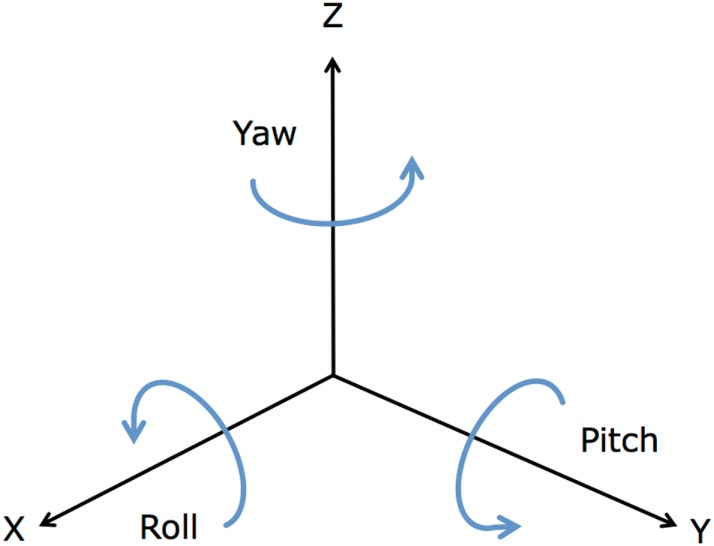
\includegraphics[width=250pt]{rpy}
\caption{world frame coordinate used in the following images}
\end{figure}

\begin{figure}[H]
\centering
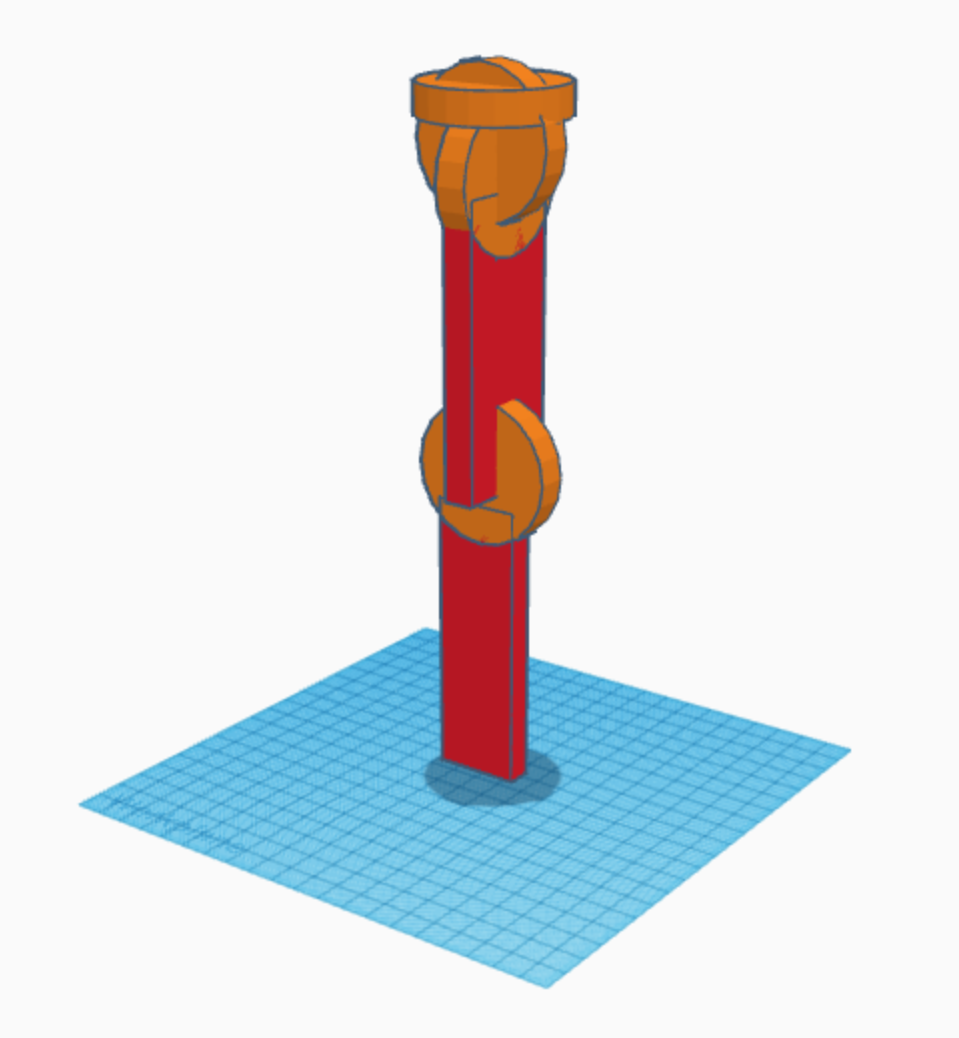
\includegraphics[width=250pt]{leg}
\caption{4 DOF (From top to bottom): Yaw at hip (+ counterclockwise),  Roll at hip (+ counterclockwise), Pitch at hip (+ counterclockwise), Roll at knee (+ counterclockwise).}
\end{figure}

Then we extract the D-H parameters from this model.

\begin{figure}[H]
\centering
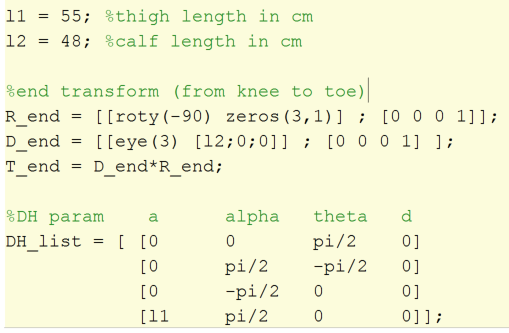
\includegraphics[width=200pt]{leg_para}
\caption{D-H parameters extracted from a human right leg.}
\end{figure}

After we compute the transformation matrices using equation:

\begin{figure}[H]
\centering
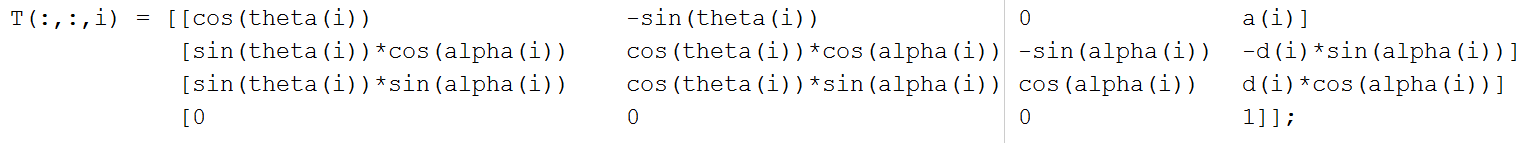
\includegraphics[width=\textwidth]{trans}
\end{figure}

We test this forward kinematics model with controlled configuration state. 

\begin{figure}[H]
\centering
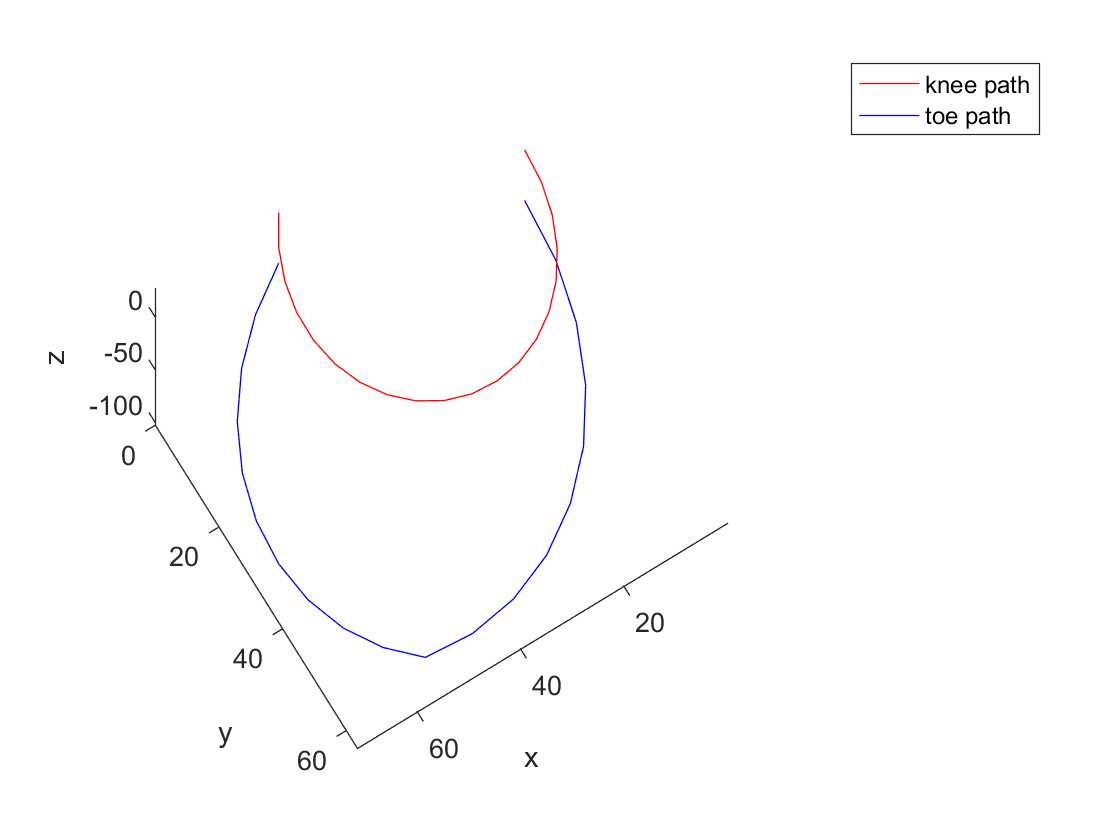
\includegraphics[width=\textwidth]{fk}
\caption{A sample kick-and-retract-to-the-side movement.}
\end{figure}

In the next part, we implement the inverse kinematics algorithm. We first created a linear path of desired operational state.

\begin{figure}[H]
\centering
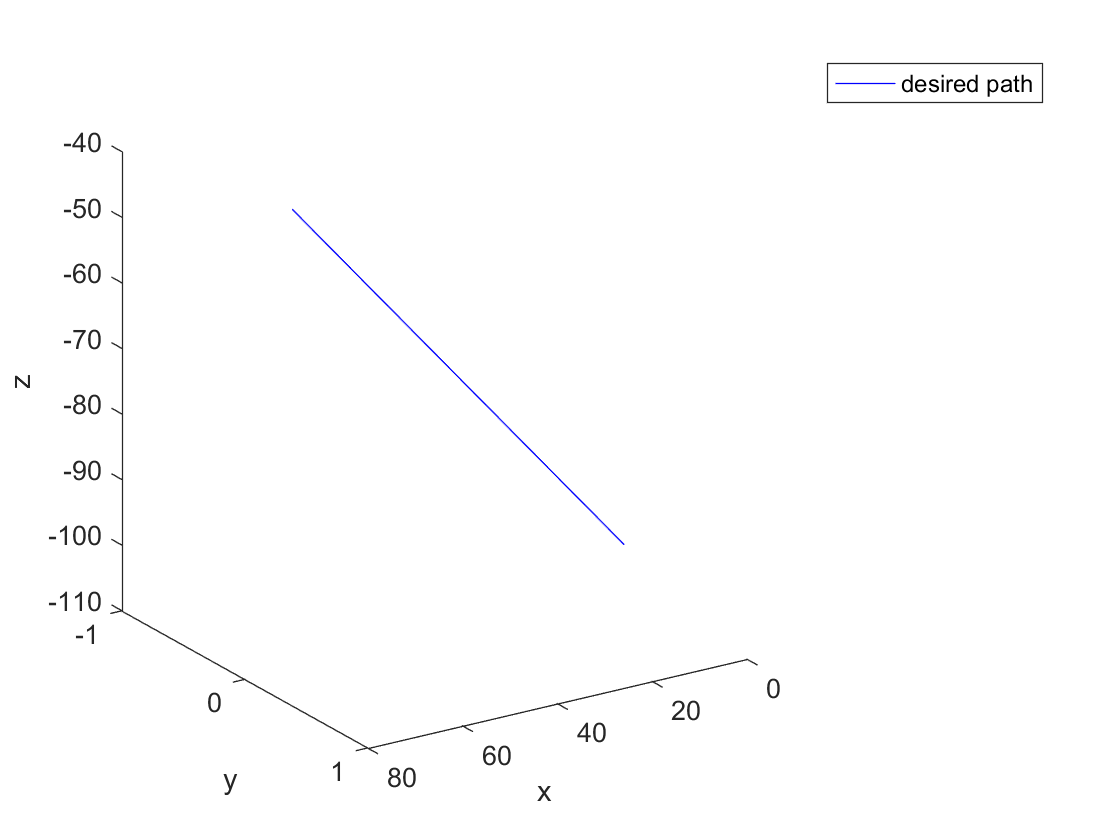
\includegraphics[width=\textwidth]{desired}
\end{figure}

Since our system is under-actuated, we only try to make the coordinates of end effector(toe) match with the path, and disregard the rotational orientation.\\
We implemented an iterative method to find the joint states given an end coordinate. First we pick a joint state, evaluate the difference between the desired joint state and the current state, calculate the Jacobian matrix, and take a joint state step forward. \\
Since this motion starts at the all-zero configuration-state, we used this as a known starting point. And for each next point, we use the previous calculated joint state values as the start searching point.

\begin{equation}
	dq = (J^TJ)^{-1}J^T \times ds 
\end{equation}

In practice, We divided each row $\vec{r}$ of the Jacobian matrix by $||\vec{r}||^2$ and multiplied it with the difference $\delta s$.

\section{Results}

We setup a threshold of error at $0.01 cm$ and it yields:

\begin{figure}[H]
\centering
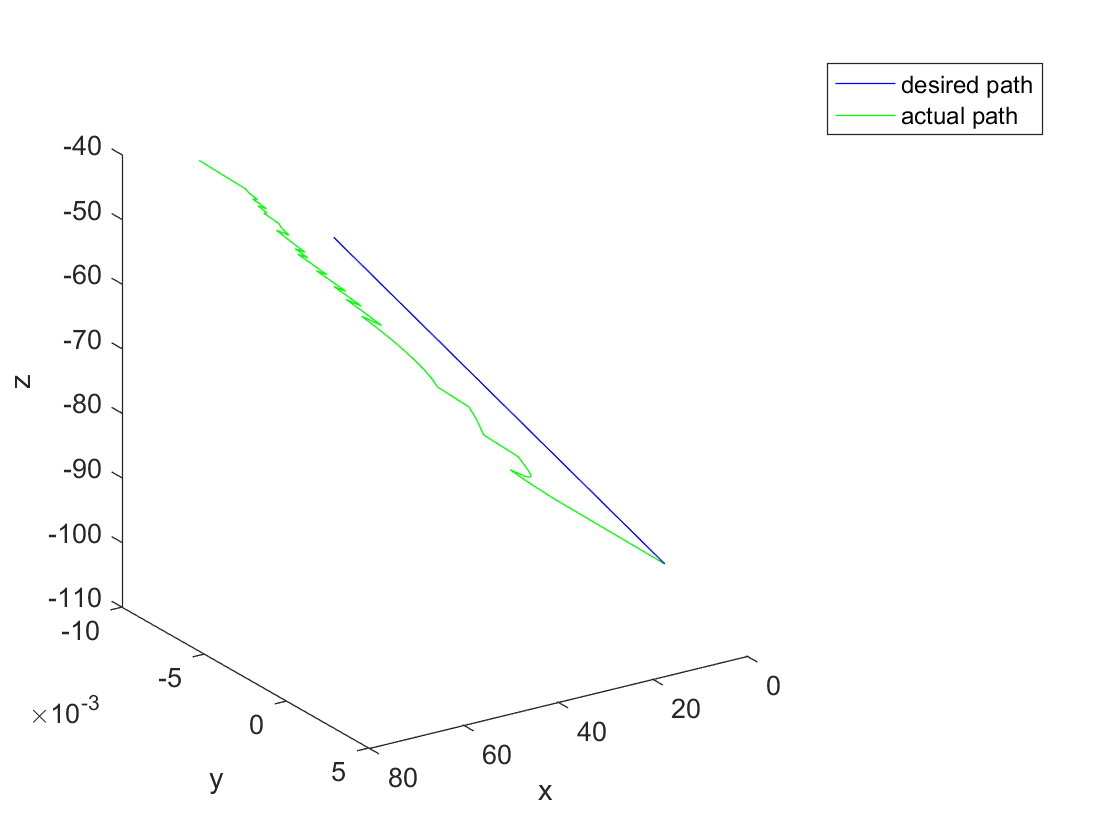
\includegraphics[width=\textwidth]{difference}
\caption{Calculated path with 0.01 cm tolerance.}
\end{figure}

The threshold can be set smaller to achieve a more accurate path.

\begin{figure}[H]
\centering
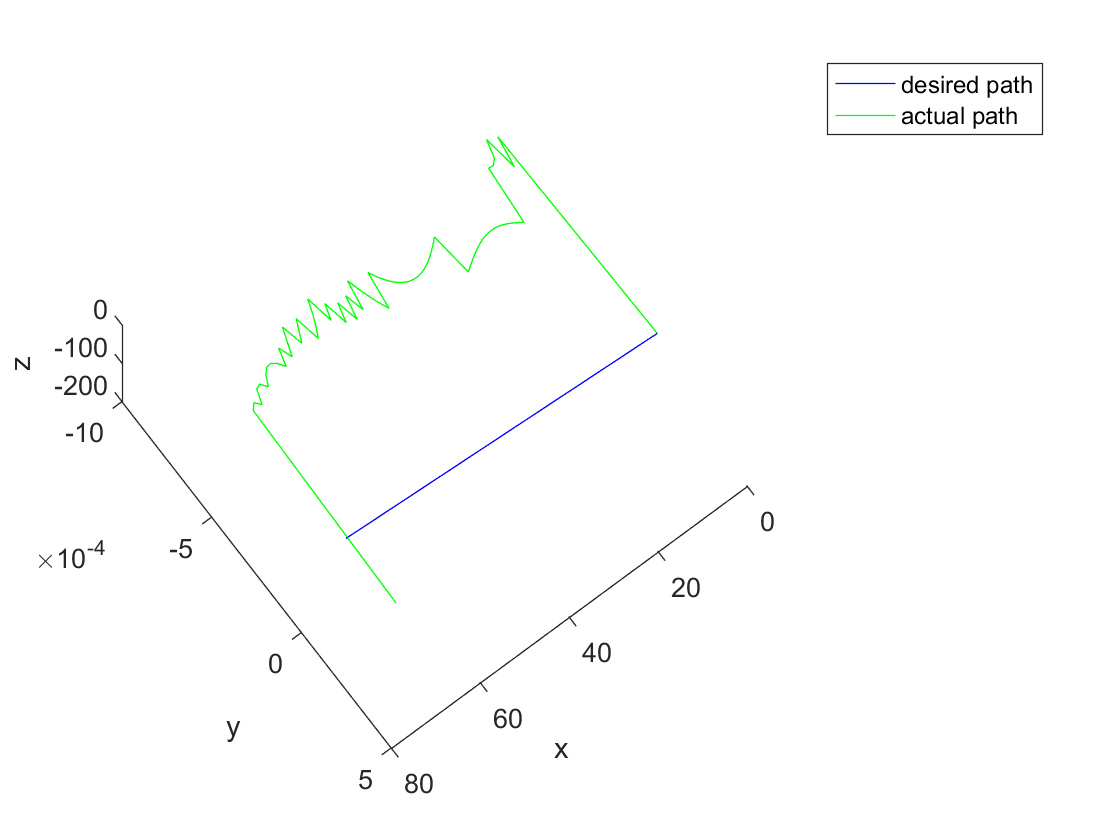
\includegraphics[width=\textwidth]{difference0_001}
\caption{Calculated path with 0.001 cm tolerance.}
\end{figure}

This lab took me about 8 hours. Debugging took about half of the time.

\end{document}

